\documentclass[11pt]{beamer}
\usepackage[utf8]{inputenc}
%\usepackage[spanish]{babel}
\usepackage{amsmath}
\usepackage{amsfonts}
\usepackage{amssymb}
\usepackage{graphicx}
\usetheme{default}
\usetheme{Madrid}
\usecolortheme{beaver}
\usepackage{textpos}
\usepackage{eso-pic}
\usepackage{mathrsfs}

\usepackage{tikz}
\usetikzlibrary{matrix}
\usetikzlibrary{snakes}
\usepackage{pgfplots}
\pgfplotsset{compat=1.12}

\newtheorem{defi}{{\it Definici\'on}}[section]
\newtheorem{thm}{{\it Teorema}}[section]

\usepackage{schemata}
\newcommand\diagram[2]{\schema{\schemabox{#1}}{\schemabox{#2}}}

\beamertemplatenavigationsymbolsempty
\setbeamertemplate{footline}[frame number]
\newcommand\AtPagemyUpperLeft[1]{\AtPageLowerLeft{
		\put(\LenToUnit{0.75\paperwidth},\LenToUnit{0.9\paperheight}){#1}}}
\AddToShipoutPictureFG{
	\AtPagemyUpperLeft{{\includegraphics[width=2.7cm,keepaspectratio]{logo}}}
}%

\AtBeginSection[]{
	\begin{frame}
		\vfill
		\centering
		\begin{beamercolorbox}[sep=8pt,center,shadow=true,rounded=true]{title}
			\usebeamerfont{title}\insertsectionhead\par%
		\end{beamercolorbox}
		\vfill
	\end{frame}
}
\usepackage{ragged2e}
\justifying

\begin{document}
	\author[Claudio Cuevas Pazos]{\includegraphics[height=2.5cm,width=5cm]{logo}\\Claudio Cuevas Pazos}
	\title{Productos Financieros Derivados}
	%\subtitle{}
	%\logo{}
	\institute{Quantitative Finance Training Center}
	%\date{}
	%\subject{}
	%\setbeamercovered{transparent}
	\setbeamertemplate{navigation symbols}{}
	\frame[plain]{\maketitle}

	
\begin{frame}{{}}
	\tableofcontents
\end{frame}


\section{Fundamentos}

\begin{frame}{Series financieras ''Aleatorias''}
	\begin{figure}
		\centering
		\includegraphics[width=.9\linewidth]{marketwatch}
		\caption{''Los mercados han sufrido gran volatilidad debido a que alguien puso un tablero de ouija en la pared NYSE controlada por el movimiento de los precios de las acciones''.}
		\label{fig:marketwatch}
	\end{figure}
	
\end{frame}

\begin{frame}{¿Qué es un derivado?}
	\begin{figure}
		\centering
		\includegraphics[width=1\linewidth]{dt150328}
		\caption{Existen muchas personas en los mercados que creen saber que es un derivado, sin embargo, entenderlos requiere de varias herramientas económicas, financieras, y sobre todo matemáticas.}
		\label{fig:dt150328}
	\end{figure}
	
\end{frame}


\begin{frame}{Fundamentos}
	Para comenzar, un derivado se define como un instrumento financiero, tal que su valor queda determinado por el valor de un instrumento financiero o no financiero, conocido como activo \textbf{subyacente}.\\
	Dichos subyacentes pueden clasificarse por el mercado al que pertenecen:
	\begin{itemize}
		\item Mercado de deuda o Renta Fija (Rates).
		\item Mercado de renta variable (Equities).
		\item Mercado de tipos de cambio (FX).
		\item Mercado de bienes renovables y no renovables (Commodities).
		\item Mercado de Crédito.
	\end{itemize}

Al existir una fluctuación diaria en los precios de estos instrumentos, las empresas se ven motivadas a asegurar los precios sobre insumos de producción, asegurar un tipo de cambio para las importaciones, asegurar una tasa de interés para un préstamo, etc.Un instrumento derivado puede verse como una \textbf{cobertura} ante ciertos factores de incertidumbre. 
\end{frame}

\begin{frame}{Uso de los productos derivados}
	
	\begin{itemize}
		\justifying
		\item Cobertura:
		Tomar una posición contraria en el instrumento derivado, tal que mitigue las pérdidas o ganancias que puedan ocurrir respecto al valor del subyacente.

		
		\item Especulación:
		Los especuladores hacen apuestas o suposiciones sobre la tendencia del mercado. Ej., si un especulador piensa que una acción está sobrevaluada, él compraría la opción de vender dicha opción en un futuro al precio de hoy, pudiendo hacer una ganancia con dicha operación.
		\item Arbitraje: Frecuentemente, ocurre en los mercados financieras que las valuaciones de ciertos instrumentos no son correctas, entonces, un participante puede aprovechar esta oportunidad para construir un portafolio que replique el precio \textbf{justo} del instrumento y hacer ganancia con ésto.
	\end{itemize}
\end{frame}

\begin{frame}{¿Dónde comprar y vender derivados?}
	En general, podemos clasificar al mercado financiero en dos grandes rubros:
	\begin{itemize}
		\item Mercados organizados
		\begin{figure}
			
			\includegraphics[width=0.3\linewidth]{NYSE-logo-2014}
			
		\end{figure}
		
		\item Mercados ''Over the Counter''
		\begin{figure}

			\includegraphics[width=0.3\linewidth]{over_the_counter}

		\end{figure}
		
		
		
	\end{itemize}
\end{frame}

\begin{frame}{Breve mención a Administración de Riesgos}
	La teoría de valuación de derivados está fuertemente relacionada con la administración de riesgos; por disposiciones regulatorias, cada banco debe contar con un equipo de administración de riesgos encargado de vigilar las operaciones que haga el banco en los mercados financieros. Dicho equipo vigila y mitiga en gran medida los siguientes riesgos:
	\begin{itemize}
		\item Riesgo de Mercado
		\item Riesgo de \textbf{Contraparte} (Diferente a Riesgo de Crédito).
		\item Riesgo de Liquidez
		\item Riesgo operativo
	\end{itemize}

En el último módulo, se verán dichos conceptos más a fondo, pero es fundamental saber la definición de los mismos, ya que se utilizaran los conceptos a lo largo de todo el curso.

\end{frame}




\begin{frame}{Motivación}
	Supongamos que en una carrera de caballos nosotros tenemos la certeza que con probabilidad de .7, nuestro caballo favorito ganará la carrera.
	\begin{center}
		
	\begin{tikzpicture}[>=stealth,sloped]
	\matrix (tree) [%
	matrix of nodes,
	minimum size=1cm,
	column sep=3cm,
	row sep=.5cm,ampersand replacement=\&
	]
	{
				\& $+1$ \&  \\
		$1$ 	\&   	 \&  \\
				\& $-1$ \&  \\
	};
	\draw[->] (tree-2-1) -- (tree-1-2) node [midway,above] {$p=\text{.}7$};
	\draw[->] (tree-2-1) -- (tree-3-2) node [midway,below]{$(1-p)=\text{.}3$};
	\end{tikzpicture}
	\end{center}

	La casa de apuestas del hipódromo está dando $ \$ $1 por cada peso apostado si nuestro caballo pierde, de mismo modo, la casa de apuestas gana un peso si pierde el caballo.
\end{frame}

\begin{frame}{{}}
	De pronto, un sujeto se acerca y te ofrece un boleto tal que paga \$100 en caso de que tu caballo preferido gane, en caso de que no gane, el sujeto no te pagará dinero. El valor de dicho boleto es de \$60.
	
	\begin{center}
		
		\begin{tikzpicture}[>=stealth,sloped]
		\matrix (tree) [%
		matrix of nodes,
		minimum size=1cm,
		column sep=3cm,
		row sep=.5cm,ampersand replacement=\&
		]
		{
			\& $100$ \&  \\
			$60$ 	\&   	 \&  \\
			\& $0$ \&  \\
		};
		\draw[->] (tree-2-1) -- (tree-1-2) node [midway,above] {};
		\draw[->] (tree-2-1) -- (tree-3-2) node [midway,below]{};
		\end{tikzpicture}
	\end{center}
	
	Ante tal negocio piensas si es redituable vender dichos boletos, por lo que te preguntas: ¿Es preferible comprar o vender los boletos?
	
	
\end{frame}


\begin{frame}{{}}
	La ganancia esperada podemos calcularla de la siguiente forma:
	\begin{center}
		$G=\text{.}7+100+\text{.}3+0=70 \ > \ 60$,
	\end{center}

Sin embargo, ésta es la ganancia que se espera en el largo plazo, ya que hacen falta de varios experimentos para que realmente observemos esas probabilidades en la vida real (de hecho bastantes...).

Si nosotros vendemos el boleto, pasa lo siguiente:
\begin{enumerate}
	\item Vendemos un boleto y recibimos \$60.
	\item Vamos a la casa de apuestas y apostamos \$50 a nuestro caballo favorito.
	\item Si ganamos, Recibimos \$100, los cuales estamos obligados a pagárselos al comprador del boleto.
	\item Si perdemos, perdemos los \$50 pero no debemos pagarle nada al comprador del boleto.
	\item Nos quedamos con \$10 !!!
\end{enumerate}
\end{frame}

\begin{frame}{{}}
	\begin{itemize}
		\justifying
		\item En el ejemplo anterior, puede verse que nuestra mejor estrategia es vender los boletos, ya que pudimos ganar dinero sin ningún riesgo en ambos escenarios. A este concepto se le conoce como \textbf{Arbitraje} y será la piedra angular de toda la teoría de valuación de instrumentos derivados.
		
		\item La idea fundamental dentro de la valuación de productos financieros derivados es construir un portafolio de réplica con los instrumentos disponibles en nuestra economía, el valor de dicho portafolio será el mismo que el valor de nuestro derivado, ya que si no lo fuera, conllevaría a una oportunidad de arbitraje
		
	\end{itemize}
	
	
	. 
\end{frame}


\section{Composición de tasas y convenciones}

\begin{frame}{Introducción}
	
	El valor del dinero en el tiempo es una idea fundamental dentro de las finanzas, como bien sabemos, hasta el dinero tiene su precio, y dicho precio se ve reflejado en las tasas de interés.
	\begin{figure}
		\centering
		\includegraphics[width=0.7\linewidth]{investing}
		
		\label{fig:investing}
	\end{figure}
	
\end{frame}


\begin{frame}{{}}
	En finanzas, hay dos maneras de capitalizar el dinero, las cuales son las siguientes:\medskip
	\medskip
	\begin{itemize}
		\item Composición simple:
		\begin{center}
			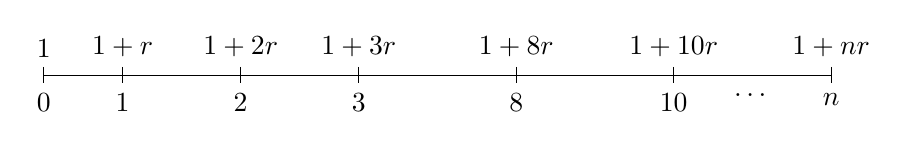
\begin{tikzpicture}
			% draw horizontal line   
			\draw (0,0) -- (2.5,0);
			\draw (2.5,0) -- (5,0);
			\draw (5,0) -- (7.5,0);
			\draw (7.5,0) -- (10,0);
			
			% draw vertical lines
			\foreach \x in {0,1,2.5,4,6,8,10}
			\draw (\x cm,3pt) -- (\x cm,-3pt);
			
			% draw nodes
			\draw (0,0) node[below=3pt] {$ 0 $} node[above=3pt] {$ 1  $};
			\draw (1,0) node[below=3pt] {$ 1 $} node[above=3pt] {$ 1+r $};
			\draw (2.5,0) node[below=3pt] {$ 2 $} node[above=3pt] {$ 1+2r $};
			\draw (4,0) node[below=3pt] {$ 3 $} node[above=3pt] {$ 1+3r $};
			\draw (6,0) node[below=3pt] {$ 8 $} node[above=3pt] {$ 1+8r $};
			\draw (8,0) node[below=3pt] {$ 10 $} node[above=3pt] {$ 1+10r $};
			\draw (9,0) node[below=3pt] {$ \dots $} node[above=3pt] {$ $};
			\draw (10,0) node[below=3pt] {$ n $} node[above=3pt] {$ 1+nr $};
			\end{tikzpicture}
		\end{center}
	
	\medskip
	\medskip
	\item Composición compuesta (Valga la redundancia...)
	\begin{center}
		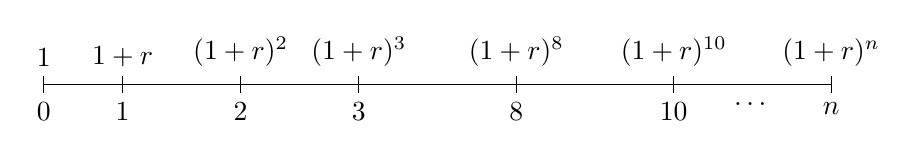
\begin{tikzpicture}
		% draw horizontal line   
		\draw (0,0) -- (2.5,0);
		\draw (2.5,0) -- (5,0);
		\draw (5,0) -- (7.5,0);
		\draw (7.5,0) -- (10,0);
		
		% draw vertical lines
		\foreach \x in {0,1,2.5,4,6,8,10}
		\draw (\x cm,3pt) -- (\x cm,-3pt);
		
		% draw nodes
		\draw (0,0) node[below=3pt] {$ 0 $} node[above=3pt] {$ 1  $};
		\draw (1,0) node[below=3pt] {$ 1 $} node[above=3pt] {$ 1+r $};
		\draw (2.5,0) node[below=3pt] {$ 2 $} node[above=3pt] {$ (1+r)^{2} $};
		\draw (4,0) node[below=3pt] {$ 3 $} node[above=3pt] {$ (1+r)^{3} $};
		
		\draw (6,0) node[below=3pt] {$ 8 $} node[above=3pt] {$ (1+r)^{8} $};
		\draw (8,0) node[below=3pt] {$ 10 $} node[above=3pt] {$ (1+r)^{10} $};
		\draw (9,0) node[below=3pt] {$ \dots $} node[above=3pt] {$ $};
		\draw (10,0) node[below=3pt] {$ n $} node[above=3pt] {$ (1+r)^{n} $};
		\end{tikzpicture}
	\end{center}
	\end{itemize}

\end{frame}

\begin{frame}{{}}
		Otra composición de tasas fundamental, es la composición pagadera $k$ veces por periodo, las cuales pueden representarse de la siguiente forma:
	\begin{equation}
	A(n)=\left(1+\frac{i^{(k)}}{k} \right)^{kn}
	\end{equation}
	 Podemos tener tasas anuales pagaderas cada 6 meses, o cada 3 meses, o cada mes, o cada semana, o cada día, o cada hora,...\medskip
	
	¿Qué pasa si la frecuencia de los pagos es tan corta que tiende a cero?
	\begin{equation}
	\label{eq:contcompound}
	\left(1+\frac{i^{(k)}}{k} \right)^{kn} \rightarrow e^{r t}
	\end{equation}
	cuando $k \rightarrow \infty$. A $r$ se le conoce como la tasa compuesta continuamente.
\end{frame}
\begin{frame}{Convenciones de conteo de días '$\alpha$'}
	Convención que se pacta para calcular el número de días que han pasado para calcular el interés devengado en una operación financiera.
	Las convenciones más usadas en los mercados financieros son las siguientes: 
	\begin{itemize}
		\item Base 30/360 : Meses de 30 días y años de 360 días.
		\item Base 30/365 : Meses de 30 días y años de 365 días.
		\item Base ACT/360: Meses con los días reales que tienen y los años de 360 días.
		\item Base ACT/365: Meses con los días reales que tienen y los años de 365 días.
		\item Base ACT/ACT: Meses con los días reales que tienen y los años con días reales que tienen.
		\item Base Business/252: Meses con los días hábiles que tienen y los años de 252 días.
	\end{itemize}
	 
\end{frame}

\begin{frame}{Convenciones de días Hábiles}
	En los mercados financieros, existen motivaciones para determinar el día en el que se paga el valor de un instrumento financiero (ya sea Nocional, cupón, payoff, etc). Existen convenciones para determinar las fechas de pago:
	\begin{itemize}
		\item No adjustment: Los pagos se efectúan en la fecha de pago (sin importar si el día es hábil o no).\medskip
		\item Previous: Si el pago cae en día inhábil, se efectúa el pago el día previo hábil inmediato a la fecha no ajustada. 
		\item Following: Si el pago cae en día inhábil, se efectúa el pago el día posterior hábil inmediato a la fecha no ajustada.\medskip
		\item Modified Previous: Convención previous, pero si el día en dicha convención cae en un mes distinto al de la fecha no ajustada, se toma el día posterior hábil inmediato perteneciente a dicho mes.
		

	\end{itemize}

\end{frame}


\begin{frame}{Convenciones de días hábiles}
	\begin{itemize}
		\item Modified Following: Convención following, pero si el día en dicha convención cae en un mes distinto al de la fecha no ajustada, se toma el día previo hábil inmediato perteneciente a dicho mes.\medskip
		\item End of Month (No Adj): Se asume que todos los pagos se efectúan al final de cada mes (sin importar si el final de mes es hábil o no).\medskip
		\item End of Month (Previous): Si el final de mes es inhábil, se toma el día previo al final de mes inmediato que sea hábil.\medskip
		\item End of Month (Following): Si el final de mes es inhábil, se toma el día posterior al final de mes inmediato que sea hábil.
	\end{itemize}
\end{frame}

\begin{frame}{Bonos}
\begin{itemize}
	\item Los bonos son instrumentos negociados en el mercado de deuda.
	\item Tienen las siguientes características:
	\begin{enumerate}
		\item Face Value $FV$
		\item Tasa Cupón $c$
		\item YTM
	\end{enumerate}
	\item Se calculan de la sig forma:
	\begin{equation}
	P_t=\sum_{i=1}^{N}D(0,t_i)C_{t_i}+FV \ D(0,t_N)
	\end{equation}
\end{itemize}
\end{frame}

\begin{frame}{Duración de Macauly }
Media ponderada de los distintos vencimientos de los flujos de caja, ponderados por el valor actual de cada uno de esos flujos.

La fórmula que resulta es:

\begin{equation}
DMac = \frac{\sum_{i=1}^{n}{t_i PV_i}} {\sum_{i=1}^{n}{PV_i}}  = \frac{\sum_{i=1}^{n}{t_i PV_i}} {V}  = \sum_{i=1}^{n}t_i \frac{{PV_i}} {V}
\end{equation}
 

donde:
\begin{itemize}
	\item $i$ es el índice de los flujos de caja,
	\item $PV_i$ es el valor actual del $i$th pago de un bono,
	\item $t_i$ es el tiempo en años que transcurre hasta el momento del $i$th pago,
	\item $V$ es el valor actual de todos los flujos de caja futuros del bono.
\end{itemize}

\end{frame}

\begin{frame}{Propiedades de la Duración}
\begin{enumerate}
	\item La duración es mayor cuanto mayor es el plazo de vencimiento del bono, aunque en menor medida que el plazo. En efecto, el valor actual más pequeño es el de los flujos o cupones que tienen su vencimiento más alejado en el tiempo.
	\item La duración de un bono es igual al plazo de amortización del título:
	\begin{itemize}
		\item En los bonos cupón cero o al descuento.
		\item Cuando solo queda un vencimiento pendiente.
	\end{itemize}
	\item Una variación importante de la duración de Macauly es la duración modificada, la cual se calcula de la siguiente forma:
	\begin{equation}
	D_m=\frac{-D_{Macauly}}{1+YTM}=\frac{\partial P}{\partial r}
	\end{equation}
\end{enumerate}
\end{frame}



\begin{frame}{Convexidad}
La convexidad es una medida que contribuye a calcular la variación y la sensibilidad del precio de un bono ante las modificaciones del tipo de interés de mercado, complementaria de la duración modificada. La duración y la convexidad sirven para estimar las variaciones de valor de un bono y constituyen herramientas valiosas para la administración del riesgo de tipo de interés.

La convexidad es la curvatura de la relación precio-rentabilidad de un bono. 
\begin{equation}
C=\frac{1}{P}  \frac{\partial^2 P}{\partial r^2}
\end{equation}
\begin{equation}
\frac{ \bigtriangleup P}{P} =
\underbrace{ D_m \bigtriangleup r }_{ Duraci \acute{o} n } +
\underbrace{ \frac{1}{2}  C \bigtriangleup r^2 }_{convexidad}
\end{equation}


\end{frame}

\section{Derivados Lineales}
\subsection{Futuros y Forwards}
\begin{frame}{Forward}
	\begin{itemize}
		\item Contrato celebrado entre dos partes, en el cual se tiene la obligación para comprar o vender un bien subyacente $S$ a precio fijado $K$ a una fecha determinada.
		
		\item Forwards más comunes: Tipo de cambio, Renta fija, Renta Variable y Commodities.
		
		\item Dos formas de liquidar los contratos de forward:
		\begin{enumerate}
			\item Por diferencias (\textit{non delivery forward}): al vencimiento del contrato se compara el tipo de cambio spot contra el tipo de cambio pactado (usualmente el forward), y el diferencial en contra es pagado por la parte correspondiente en la moneda local o extranjera.
			\item Por especie (\textit{delivery forward}): al vencimiento el comprador y el vendedor intercambian las monedas según el tipo de cambio pactado.
			
		\end{enumerate}
		
	\end{itemize}
	
	Payoff:
	\begin{equation}\label{fwd:payodd}
	V_T=(S_T-K)
	\end{equation}
\end{frame}

\begin{frame}{{}}
	\begin{itemize}
		\item La pregunta complicada en este tipo de instrumentos es: cómo valuarlos?
		\item La solución dada a este problema es utilizando como fundamento el concepto de no arbitraje. Nuestro propósito será encontrar un portafolio tal que dada una estrategia podamos replicar el payoff del derivado. A este portafolio se le conoce como portafolio de cobertura y el precio del derivado necesariamente tendrá que coincidir con el del portafolio de cobertura.
		\item Definamos la economía consistente en un activo de renta variable $S_t$ y un activo de renta fija $D_{tT}$, el segundo se define de la siguiente forma:
		\begin{equation}
		dD_{tT}=rD_{tT} dt,
		\end{equation}
		donde $r$ se define como la tasa libre de riesgo. Normalmente a $D_{tT}$ se le conoce como la cuenta corriente.
	\end{itemize}
	
\end{frame}

\begin{frame}{{}}
	Recordemos que el significado de la ecuación \ref{fwd:payodd} es la compra de un bien a precio $K$ pactado al inicio del contrato. Bajo el concepto de no arbitraje, supongamos que al tiempo $t$ entramos en un contrato forward largo. En el cual nos comprometemos a comprar $S_t$ a una cantidad  de dinero $K$, si a este contrato forward le añadimos la cantidad $K$, al  tiempo $T$ tendremos el siguiente payoff:
	\begin{equation}
	\widehat{V}_T^{(1)}=f_T+K=(S_T-K)+K=S_T
	\end{equation} 
	Como portafolio de cobertura, necesitamos un portafolio que genere el mismo payoff al tiempo $T$. Si utilizamos 
	\begin{equation}
	\widehat{V}_T^{(2)}=S_T,
	\end{equation}
	Tendremos un portafolio de cobertura Bajo el concepto de no arbitraje (o ley de un solo precio), ambos portafolios deben tener el mismo valor en $t$, es decir:
	\begin{equation}
	f_t+D_{tT} K=S_t
	\end{equation}
\end{frame}

\begin{frame}{{}}
	Esto pasa si y solo si:
	\begin{equation}\label{fwd:price}
	f_t=S_t-D_{tT}K.
	\end{equation}
	Una de las definiciones importantes es el \textit{precio forward} de un derivado, el cual es la $K$ tal que hace que el valor del contrato forward sea 0. En este caso, igualamos el lado derecho de la ecuación (\ref{fwd:price}) a 0 y tenemos que:
	\begin{equation}
	F_t=D_{tT}^{-1}S_t
	\end{equation}
	
	
\end{frame}



\begin{frame}{Forward de tipo de cambio}
	En los Forwards de tipo de cambio, a vencimiento $T$, se intercambian flujos de efectivo en distintas divisas. En otras palabras, al inicio del contrato se pacta un tipo de cambio $K$ tal que se intercambiarán los flujos de dinero a dicho tipo de cambio. Para encontrar el tipo de cambio forward, considerar lo siguiente:
	\begin{enumerate}
		\item Teniendo una cantidad de dinero en moneda extranjera $N^{fx}$ a tiempo $t$, podemos crear dos estrategias:
		\begin{itemize}
			\item Comprar moneda local al tipo de cambio Spot e invertir dicho dinero a la tasa libre de riesgo local $r_{loc}$, resultando en $X_T^{(1)}=N^{fx}*S_0* e^{r_{loc}(T-t)}$.
			\item Invertir $N^{fx}$ a la tasa libre de riesgo extranjera $r_{fx}$ y a vencimiento, convertir el monto final al tipo de cambio pactado $K$, resultando en $X_T^{(2)}=N^{fx}*K* e^{r_{fx}(T-t)}$
		\end{itemize}
	\item Los dos portafolios tienen el mismo valor inicial que es $N^{fx}$, por lo que al no haber riesgo involucrado, ambos portafolios deben valer lo mismo, por lo que llegamos a la siguiente relación:
	\begin{equation}
	S_0 e^{r_{loc}(T-t)}=K e^{r_{fx}(T-t)}
	\end{equation}
	\end{enumerate}
\end{frame}
\begin{frame}{{}}
	El resultado anterior solo es aplicable para el tipo de cambio forward, sin embargo, podemos utilizar un argumento similar para encontrar el valor de un contrato forward con cualquier strike $K$ (i.e. el payoff es $N(S_T-K)$):
	\begin{enumerate}
		\item Pactar un forward Largo e invertir $NKe^{-r_{loc}}$ unidades de dinero local. 
		\item Invertir $Ne^{-r_{fx}}$ unidades de dinero extranjero.
		\item A tiempo $T$, tendremos que el primer portafolio vale $NS_T-NK+NK=NS_T$ unidades de dinero local.
		\item Al tiempo $T$, tendremos que el segundo portafolio vale $N$ unidades de dinero extranjero, o $NS_T$ unidades de dinero local.
		\item Bajo el supuesto de no arbitraje, ambas estrategias dan el mismo payoff, por lo que el valor a tiempo $t$ de ambas debe ser igual, es decir:
		\begin{equation}
		f_t=N(e^{-r_{fx}}S_t-Ke^{-r_{loc}})
		\end{equation}
	\end{enumerate}
\end{frame}

\begin{frame}{{}}
	\begin{figure}
		\centering
		\includegraphics[width=0.7\linewidth]{6-eur-frd-screenshot}
		\caption{Cotizaciones de Forwards de tipo de cambio en Mercado}
		\label{fig:6-eur-frd-screenshot}
	\end{figure}
\end{frame}

\begin{frame}{FRA's}
Un FRA o \textit{Forward Rate Agreement} es un acuerdo entre dos contrapartes, en el que intercambian dos flujos de dinero en el futuro.\medskip
Componentes:
\begin{itemize}
	\item Nocional $N$
	\item Fecha de Fixing $T$
	\item Fecha de pago $S$
\end{itemize}
	El payoff de dicho instrumento es e siguiente:
	\begin{equation} \label{payofffra}
	X_T=\alpha N (L_T[T,S]-K)
	\end{equation}
	\begin{center}
		\begin{tikzpicture}
		% draw horizontal line   
		\draw (0,0) -- (8,0);
		
		% draw vertical lines
		\foreach \x in {0,4,8}
		\draw (\x cm,3pt) -- (\x cm,-3pt);
		\draw (0,0) node[below=3pt] {$ 0 $} node[above=3pt] {$   $};
		\draw (4,0) node[below=3pt] {$ T $} node[above=3pt] {$  $};
		\draw (8,0) node[below=3pt] {$ S $} node[above=3pt] {$ 1+\alpha L_{T}[T,S] $};
		\draw (8,0) node[below=15pt] {$ 1+\alpha K $} node[above=3pt] {$  $};
		
		\end{tikzpicture}
		
	\end{center}
\end{frame}

\begin{frame}{Valuación de un FRA}
	Podemos modificar la ecuación \eqref{payofffra}, con el fin de verla como la diferencia de dos bonos cupón cero:
	\begin{equation}\label{pricefra}
	X_T=N(1+\alpha L_T[T,S])-N(1+\alpha K)
	\end{equation}
	De la ecuación anterior es más fácil intuir cómo replicar dicho payoff utilizando bonos cupón cero.\medskip
	Tomando el portafolio
	\begin{equation}
	V_t=D_{tT}-(1+\alpha K)D_{tS},
	\end{equation}
	
	del primer bono cupón cero que compramos, a tiempo $T$, invertimos la unidad monetaria obtenida a tasa $L_T[T,S]$, y del segundo bono  cupón cero que vendimos esperamos hasta $S$ ara recibir $(1+\alpha K)$, el valor del portafolio en $S$ coincide con \eqref{payofffra}, por lo que bajo el supuesto de no arbitraje, el valor de un FRA queda dado por la ecuación \eqref{pricefra}.
	
\end{frame}


\subsection{Swaps}
\begin{frame}{Swaps}
	
	\begin{itemize}
		\item Una de las preocupaciones más grandes de una compañía es la incertidumbre acerca del pago de sus deudas futuras.
		\item Lo anterior debido a que el valor del dinero en el tiempo, al igual que cualquier instrumento, va cambiando. Es por esto que surge la necesidad de pactar un Swap.
		\item Un Swap es un acuerdo OTC entre dos contrapartes, tal que se comprometen a intercambiar flujos de dinero en fechas futuras del tiempo, los cuales son capitalizados a tasas distintas.
		
	\end{itemize}
	\begin{center}
	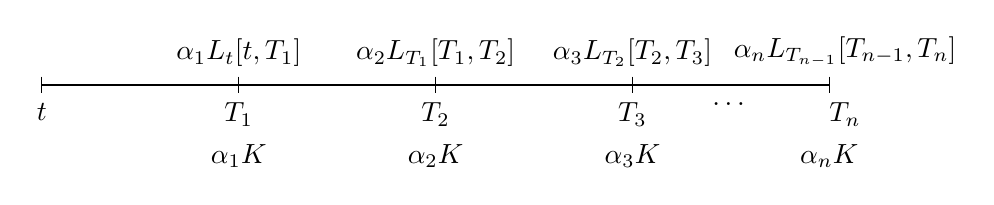
\begin{tikzpicture}[snake=zigzag, line before snake = 5mm, line after snake = 5mm]
	% draw horizontal line   
	\draw (0,0) -- (10,0);
	
	% draw vertical lines
	\foreach \x in {0,2.5,5,7.5,10}
	\draw (\x cm,3pt) -- (\x cm,-3pt);
	
	% draw nodes
	\draw (0,0) node[below=3pt] {$ t $} node[above=3pt] {$   $};
	\draw (2.5,0) node[below=3pt] {$ T_1 $} node[above=3pt] {$ \alpha_1 L_{t}[t,T_1] $};
	\draw (2.5,0) node[below=18pt] {$ \alpha_1 K $} node[above=3pt] {$  $};
	\draw (5,0) node[below=3pt] {$T_ 2 $} node[above=3pt] {$ \alpha_2 L_{T_1}[T_1,T_2]  $};
	\draw (5,0) node[below=18pt] {$ \alpha_2 K $} node[above=3pt] {$  $};
	\draw (7.5,0) node[below=3pt] {$ T_3 $} node[above=3pt] {$ \alpha_3 L_{T_2}[T_2,T_3]  $};
	\draw (7.5,0) node[below=18pt] {$ \alpha_3 K $} node[above=3pt] {$  $};
	\draw (8.75,0) node[below=3pt] {$ \dots $} node[above=3pt] {$ $};
	\draw (10.2,0) node[below=3pt] {$ T_n $} node[above=3pt] {$ \alpha_n L_{T_{n-1}}[T_{n-1},T_n]  $};
	\draw (10,0) node[below=18pt] {$ \alpha_n K $} node[above=3pt] {$  $};

	\end{tikzpicture}
\end{center}
\end{frame}

\begin{frame}{Tipos de Swaps}
	En el mercado OTC, existen distintos tipos de Swaps, los más relevantes son los siguientes:\bigskip
	
	
	\diagram{Swaps}
	{- \diagram{IRS}{- Fixed-Floating \\ - Tenor \\ \ldots} \\
		
		- \diagram{XCCY}{- Fixed-Floating \\ - Fixed Fixed \\-Basis  \\ \ldots}\\
		
		-OIS
		
	}
\end{frame}

\begin{frame}{Definición de un IRS Swap}
	Instrumento OTC de intercambio de flujos de naturaleza distinta entre las partes involucradas en el contrato.
	
	El estándar de mercado es intercambiar flujos periódicos a tasa fija por flujos periódicos a tasa variable.
	
	Al pactar una operación IRS estándar  debe definirse lo siguiente:
	\begin{itemize}
		\item Monto Nominal
		\item Tiempo a vencimiento
		\item Para la Pata Fija:
		\begin{itemize}
			\item  Tasa fija
			\item Periodicidad de pago de intereses
			\item Convención de conteo de días para pago de intereses
		\end{itemize}
		
		\item Para la Pata Flotante:
		\begin{itemize}
			\item Tasa variable de referencia (activo subyacente del IRS)
			\item Periodicidad de pago(regularmente el mismo que el tenor de la tasa referencial)
			\item Convención de conteo de días para pago de intereses
			\item Forma de revisión de la tasa flotante (reg. Fija al inicio y paga al final del periodo)
		\end{itemize}
		
		
	\end{itemize}
\end{frame}

\begin{frame}{Convenciones de IRS Swaps}
	\begin{figure}
		\centering
		\includegraphics[width=0.7\linewidth]{quotes_swaps}
		\label{fig:quotesswaps}
	\end{figure}
	
\end{frame}

\begin{frame}{USD IRS Libor3M (semiannual)}
	\begin{figure}
		\centering
		\includegraphics[width=0.7\linewidth]{USDLIBOR3MSWAP}
		\caption{Cotizaciones a distintos plazos para un IRS Libor3M}
		\label{fig:usdlibor3mswap}
	\end{figure}
	
\end{frame}

\begin{frame}{MXN IRS TIIE28D}
	\begin{figure}
		\centering
		\includegraphics[width=0.8\linewidth]{MXNTIIESWAP}
		\caption{Cotizaciones a distintos plazos para un IRS TIIE 28D}
		\label{fig:mxntiieswap}
	\end{figure}
	
\end{frame}

\begin{frame}{Interest Rate Tenor Basis  Swap}
	\begin{itemize}
	\item Swap Flotante- Flotante.
	\item Es un instrumento de intercambio de flujos, ambas patas están referenciadas a tasas flotantes denominadas en una sola moneda.

	\item Son llamados Basis Swaps porque involucran flujos en dos bases distintas dentro de una misma divisa, por ejemplo, USD-Libor3M y USD-Libor6M, esto es, en un basis swap se intercambian flujos de Libor3M por flujos de Libor6M.
	
	\item Una de las patas paga su índice referencial más un spread, el basis spread $b_T$.
	
	\begin{equation}
	\sum_{i=1}^{n}(L_i^{ST}+b_T)D_{t,t_i} \tau(t,t_i)= \sum_{j=1}^{m}L_i^{LT}D_{t,t_j} \tau(t,t_j)
	\end{equation}
	
	\end{itemize}
	 
	
	
	
	
	
\end{frame}

\begin{frame}{Overnight Indexed Swap - OIS}
	\begin{itemize}
		\item Instrumento OTC, en el que se intercambian flujos basados en  tasas fijas por flujos flotantes ligados a tasas ON.
		Lo común es que los flujos fijos y flotantes ocurran en la misma fecha.
		\item Típicamente,  si un OIS es de menos de un año, se tiene un único intercambio a vencimiento. 
		\item Si es mayor a un año los flujos se intercambian anualmente.
	\item El pago en la tasa flotante se calcula con base en la composición de acumulaciones diarias del índice ON de referencia.
	\item EL índice ON es igual a la media geométrica del tipo overnight sobre cada día del período de pago.
		\item El índice ON es típicamente un tipo de interés considerado menos arriesgado que su correspondiente tipo interbancario (LIBOR).
	\end{itemize}
\end{frame}

\begin{frame}{Convenciones de un OIS Swap}
	\begin{figure}
		\centering
		\includegraphics[width=1\linewidth]{OISQUOTES}
		\label{fig:oisquotes}
	\end{figure}
	
\end{frame}

\begin{frame}{USD OIS}
	\begin{figure}
		\centering
		\includegraphics[width=.8\linewidth]{USDOIS}
		\caption{Cotizaciones de OIS Swaps}
		\label{fig:usdois}
	\end{figure}
	
\end{frame}

\begin{frame}{Cross Currency Basis Swap \textit{XCCY}}
	\begin{itemize}
		\item Instrumento OTC donde se intercambian flujos (usualmente nominales y flujos de interés) en una divisa dada por flujos denominados en otra divisa.
		\item Lo común es que cada pata pague flujos basados en tasas flotantes, aunque puede haber tasas fijas involucradas en los pagos.
		\item Una de las patas paga su índice referencial más un spread, el cross currency basis spread.
		\item El xccy basis spread es pensando como la prima que es cargada por la diferencia de liquidez entre divisas (el costo de convertir una moneda a otra).
		\item Existen swaps resetteables y no resetteables. El primero indica que existen ajustes intercupón de nominal por movimientos en el tipo de cambio. El segundo no considera tales ajustes.
		
	\end{itemize}
\end{frame}


\begin{frame}{Cotización de un CCS USD MXN}
\begin{figure}
	\centering
	\includegraphics[width=0.8\linewidth]{CCSUSDMXN}
	\caption{Cotización de un Cross Currency basis Swap a distintos vencimientos.}
	\label{fig:ccsusdmxn}
\end{figure}

\end{frame}
\begin{frame}{Valuación de un IRS Swap}
	Hasta este momento, asumiremos que existe solamente una curva para estimar las tasas forward y para descontar los flujos futuros. En el futuro relajaremos este supuesto.\\
	
	Podemos ver a un IRS Swap como un portafolio de FRA's, sin embargo, utilizaremos otro método de valuación más directo, el cual consiste valuar las patas por separado:
	
	La pata fija consiste en una serie de pagos fijos en las fechas $T_1, T_2, \dots T_n$, cada pago de valor $\alpha K$, el valor de dicha pata puede calcularse de la siguiente forma:
	\begin{equation}
	V_t^{Fix}=K \sum_{i=1}^{n} \alpha _i D_{t T_i} := KP_t
	\end{equation}
	 A $P_t$ le llamaremos el \textit{valor presente de un punto básico} o $PVBP$ de un swap.

\end{frame}
\begin{frame}{Valuación de un IRS Swap}
		Teniendo el valor de la pata fija, resta con calcular el valor de la pata flotante para poder valuar el Swap, para ésto, consideremos un portafolio conformado por los siguientes instrumentos:
	\begin{equation}\label{eq:swap}
	V_t=1-D_{t T_n}
	\end{equation}
	
	
	\begin{enumerate}
		\item Tomemos el valor en dinero de este portafolio, podemos invertir \$1 a $T_1$ y vendamos un bono cupón cero que vence en $T_n$.
		\item Llegado el tiempo $T_1$, recibimos  $1+\alpha_1 L_{t}[t,T_1] $ por el peso invertido.
		\item Tomamos \$1 y lo volvemos a invertir de $T_1$ a $T_2$.
		\item Repitamos este proceso iterativamente hasta llegar a $T_n$
		\item En $T_n$ recibimos $1+\alpha_{n-1} L_{T_{n-1}}[T_{n-1},T_{n}] $, y a la vez tenemos que pagar \$1 derivado del bono $D_{tT_n}$.
		\item Con la estrategia anterior hemos replicado el valor de la pata flotante de un IRS!!!
	\end{enumerate}
\end{frame}

\begin{frame}{Valuación de un IRS Swap}
Solo queda calcular el valor del Swap de la siguiente forma:
\begin{eqnarray}\label{eq:swap2}
V_t^{Swap}&=&V_t^{Flt}-V_t^{Fix}\\
		  &=&1-D_{tT_n}-KP_t,
\end{eqnarray}

De las ecuaciones anteriores, podemos preguntarnos al igual que en los FRA's, cuál es el Strike tal que hace el Valor de mi Swap cero al comienzo del contrato? Despejando:
\begin{equation}\label{parswap}
y_t:=\frac{1-D_{tT_n}}{P_t}
\end{equation}

A $y_t$ se le conoce como la tasa \textit{par swap} y ésta es la que cotiza en mercado.

Sustituyendo \eqref{parswap} en \eqref{eq:swap2}, llegamos a la expresión más usual para un swap:
\begin{equation}
V_t^{swap}=P_t(y_t-K)
\end{equation}
\end{frame}
\section{Curvas de tasas de interés}
\begin{frame}{Curvas Zero Coupon}
	\begin{itemize}
		\item Sea $r(t_0,T)$ una tasa cero cupón en alguna de las composiciones definidas anteriormente.
		
		\item La función $T \rightarrow r(t_0,T)$ es llamada curva cero cupón. También es referida como la estructura temporal de tasas de interés.  
		
		\item \textbf{Importante}: Para el uso de esta función debe especificarse la composición de la tasa y la convención de conteo asociada.
		
		\item El concepto curva y estructura temporal es utilizado en un sentido mucho más amplio en las  prácticas de mercado, donde $r(,)$ puede referir además a tasas swap, el mismo factor de descuento, volatilidades, tasas de inflación o algún otro precio de mercado. En general se refiere a cualquier mapeo de un plazo con una variable de mercado.
		
	\end{itemize}
\end{frame}
\begin{frame}{Curva de Tasas Swap y Cero Cupón}
	\begin{figure}
		\centering
		\includegraphics[width=.9\linewidth]{swap_curve}
		
		\label{fig:swapcurve}
	\end{figure}
\end{frame}

\begin{frame}{Tasas de Referencia}
	\begin{itemize}
		
	
	\item En el caso de los participantes del mercado financiero mexicano, el nivel promedio de tasa de fondeo está definido por la TIIE-28D.
	
	\item Es la tasa pagada en depósitos a 28 días, por tanto útil para descontar flujos futuros \footnote{asociados a un contrato sin respaldo de colateral.} a tal plazo…
	
\item 	Y para descontar a cualquier otro plazo? Por ej, a 10Y ?
	
	\item La economía mexicana cuenta con TIIE91D y TIIE182D, pero no son referencias líquidas. Aún con eso, sólo tenemos tres tasas para definir la curva, pero…
	
	\item Existen instrumentos líquidos en los mercados que permiten definir las expectativas evolutivas de una tasa referencial (IRS de TIIE28D en el caso mexicano), de manera que puede deducirse su estructura temporal.
	
\end{itemize}
\end{frame}

\section{Construcción Clásica de las curvas de tasas de interés (Valuación sin inclusión de colaterales)
}
\begin{frame}{Bootstrapping}
	\begin{itemize}
		\item El procedimiento para inferir la curva de descuento a partir de cotizaciones líquidas del mercado se llama bootstrapping y consiste en un proceso de solución iterativo que reutiliza la información del corto plazo para generar información a más largo plazo.
		\item Es necesario establecer supuestos de interpolación y extrapolación pues sólo se cuenta con un número reducido de instrumentos.
		\item 	Lo anterior significa que existen múltiples soluciones de curva, pero toda solución válida deberá ser consistente con los precios de mercado, ie, la curva cero cupón deberá recuperar los precios de mercado de los instrumentos utilizados para su construcción.
	\end{itemize}
	
\end{frame}
\begin{frame}{Bootstrapping}
	Las fechas asociadas a la maduración de los instrumentos utilizados para bootstrappear la curva de descuento son conocidos como los pilares de construcción. \medskip

	La solución de la curva deberá ser presentada como una función $D_{0,T}$ definida a tramos, de valores dados para los $T$ que son pilares de construcción y para cualquier otro $T$ deberá generarse vía la regla de interpolación elegida.\\

	Como ejemplo, tenemos una fórmula cerrada para el valor de un IRS Swap. Con el fin de hallar los factores de descuento que hacen $0$ el valor del swap, podemos utilizar un método númerico con este fin (Newthon Rhapson).
	
\end{frame}

\begin{frame}{Bootstrapping}
	\begin{figure}
		\centering
		\includegraphics[width=1\linewidth]{bootstrapinterp}
		\caption{Ejemplo de interpolación para factores de descuento.}
		\label{fig:bootstrapinterp}
	\end{figure}
	
\end{frame}

\begin{frame}{Bootstrapping}
	\centering
	\begin{figure}
		\centering
		\includegraphics[width=\linewidth]{irs28mxn}
		\caption{Caso MXN: IRS TIIE28}
		\label{fig:irs28mxn}
	\end{figure}
	
\end{frame}

\begin{frame}{{}}
	\begin{figure}
		\centering
		\includegraphics[width=0.7\linewidth]{bloombirs}
		\caption{Ejemplo de una pantalla de cotización para un IRS Swap sobre TIIE28D}
		\label{fig:bloombirs}
	\end{figure}
	
\end{frame}


\begin{frame}{Bootstrapping Curva TIIE28D}
	Dado que los IRS de pantalla valen cero por definición, se tiene que:
	\begin{eqnarray*}
	&& V^{Fix}_{t_0}=V^{Float}_{t_0}\\
	&\iff& \sum_{i=1}^{n}N K \tau(t_{i-1}, t_{i}) D_{t_0,t_i}=\sum_{i=1}^{n}N F_0(t_{i-1},t_i) \tau(t_{i-1}, t_{i}) D_{t_0,t_i}\\
	&\iff& \sum_{i=1}^{n} K \tau(t_{i-1}, t_{i}) D_{t_0,t_i}=1-D_{t_0,t_n}\\
	&\iff & \sum_{i=1}^{n} K \tau(t_{i-1}, t_{i}) D_{t_0,t_i} +D_{t_0,t_n}=1
	\end{eqnarray*}
	
\end{frame}
\section{Construcción bajo valoraciones asociadas al colateral (Nuevo estándar de mercado)}
\begin{frame}{Evolución del Mercado Post Credit-Crunch}
Antes de 2007:
	\begin{itemize}
		\item Un FRA podía ser replicado con un par de depósitos.
		\item	Tasas forward no diferían significativamente de las calculadas teóricamente mediante tasas OIS.
	\item	El basis entre tasas de depósito y OIS era pequeño e ignorado
	\item	El basis entre tasas swap de un mismo vencimiento pero ligadas a subyacentes de tenors distintos también era ignorado, por tanto un bono flotante se negociaba a par independientemente del tenor del subyacente: Libor3M, Libor6M.
	\item El mercado no reflejaba en los precios de los swaps la posibilidad del incumplimiento de la contraparte.
		
	\item	El tratamiento consistente de los participantes de mercado sobre los puntos  anteriores permitía definir una única curva cero cupón (con la que se estiman los índices y al mismo tiempo descuentan flujos futuros)
	\end{itemize}
\end{frame}

\begin{frame}{Evolución del Mercado Post Credit-Crunch}
	Durante y posterior a la crisis iniciada en 2007:
	
	\begin{itemize}
		\item Comenzaron a ser más comunes los trades bajo acuerdos de colateral y otros mitigantes a la exposición del riesgo de contraparte (considerados contractualmente en los términos de los ISDA-CSAs )
		\item Los spreads mencionados anteriormente comenzaron a ser notorios y cada vez mayores.
		\item Se comenzaron a pagar primas altas de crédito/liquidez en fondeos interbancarios basados en Libor.
		\item Las primas  de riesgo en las tasas Libor mostraban distintas proporciones a distintos tenors, de hecho mayores a mayor plazo.
		\item La cobertura de instrumentos indizados a un subyacente dado, por ej Libor3M, se hacía solo mediante instrumentos vanillas ligados al mismo índice.
		
	\end{itemize}
\end{frame}

\begin{frame}{Evolución del Mercado Post Credit-Crunch}
	Una conclusión directa es que los índices Libor ya no eran una buena aproximación para representar una tasa libre de riesgo. En todo caso, una mejor aproximación lo son las tasas \textit{OIS} pues éstas tasas no son afectadas por primas de riesgo de crédito, dado que los \textit{OIS} swaps están sujetos a llamadas de margen diarios.
	
	Una proporción significativa de los deals bajo acuerdos ISDA comenzaron a sujetarse a llamadas de colateral (diarias  en muchos casos) las cuales son remunerados a tasas \textit{ON}.
	
	Los “precios de pantalla“ comenzaron a ser considerados  completamente colateralizados (threshold=0). 
	
	Se generó, por tanto, la necesidad de diferenciar entre curvas para la estimación de índices y consecuentemente la necesidad de generar otra referencia para el descuento basada en una nueva curva libre de riesgo y el colateral asociado a la operación: curva \textit{OIS}.
	
\end{frame}
\begin{frame}{Overnight Index Swaps (OIS)}
	\begin{itemize}
		\item 
		Overnight Index Swaps (OIS) son instrumentos que permiten a las instituciones financieras intercambiar los tipos de interés que están pagando sin tener que refinanciar o cambiar los términos de los préstamos que han tomado de otras instituciones financieras. 
		\item Cuando dos instituciones financieras pactan un swap (OIS), una de las instituciones está intercambiando una tasa de interés a un día y la otra institución está intercambiando una tasa de interés fija a corto plazo.
		\item la tasa OIS se calcula diariamente con base en el promedio de las tasas de interés que las instituciones bancarias pagaron ese día.
		\item El colateral de dichos contratos es revisado diariamente, por lo que dicha tasa puede ser considerada como la más próxima a la tasa libre de riesgo.
	\end{itemize}
\end{frame}
\section{Opciones}
\begin{frame}
Una opción es un contrato en el que alguna de las contrapartes tiene el derecho, mas no la obligación de adquirir un producto $S_t$ a un precio pactado $K$. \bigskip

\diagram{Opciones}
{- \diagram{Plain Vanilla}{- Call   $max (S_T-K,0)$ \\ - Put   $max (K-S_T,0)$} \\
	
	- \diagram{Exóticas}{- Americanas \\ - Digitales \\-Asiáticas \\-Lookback \\ \ldots}

}
En las opciones mencionadas anteriormente siempre habrán dos posiciones: La larga y la corta.
\end{frame}




\begin{frame}{Cotizaciones de opciones sobre Equity}
	
\begin{figure}
	\centering
	\includegraphics[width=.8\linewidth]{OMON_MSFT}
	\caption{Pantalla Obtenida de Bloomberg, mostrando las cotizaciones de opciones sobre la acción de Microsoft.}
	\label{fig:omon-msft}
\end{figure}

	
\end{frame}


\begin{frame}{Payoff de un Call Europeo}
	\centering
	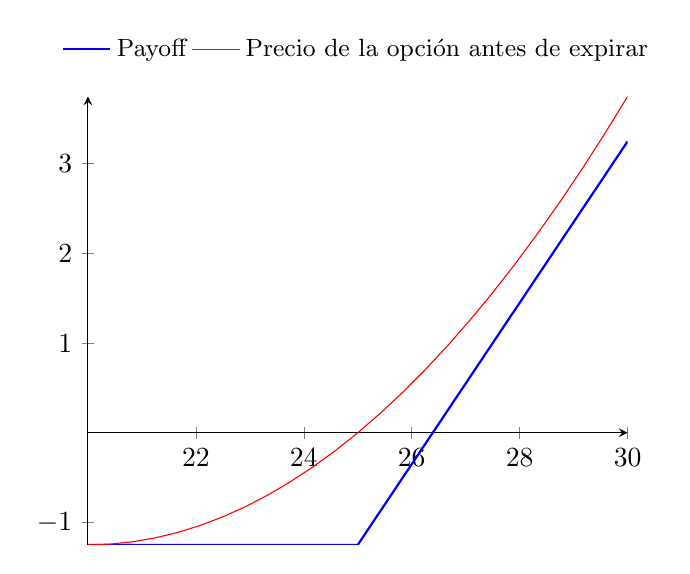
\begin{tikzpicture}[
	declare function={
		mypl(\x)= -1.25 + (\x>25) * (0.9*(\x-25));
	}
	]
	\begin{axis}[
	domain=20:30,
	axis lines=middle,
	legend style={
		draw=none,
		legend columns=-1,
		at={(0.5,1)},
		anchor=south,
		outer sep=1em,
		node font=\small,
	},
	]
	\addplot[blue,thick] {mypl(x)};
	\addlegendentry{Payoff}
	\addplot[red] {0.05*(20-x)^2-1.25};
	\addlegendentry{Precio de la opción antes de expirar};
	\end{axis}
	
	\end{tikzpicture}
\end{frame}

\begin{frame}{Payoff de un Put Europeo}
	\centering
	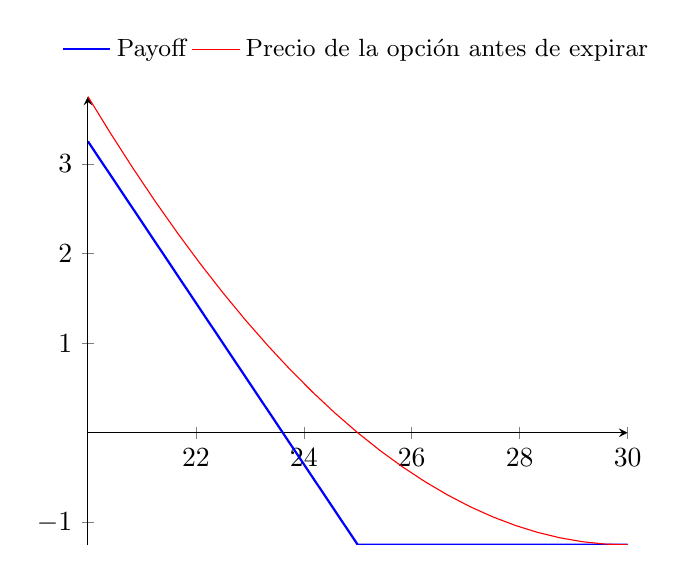
\begin{tikzpicture}[
	declare function={
		mypl(\x)= -1.25 + (\x<25) * (0.9*(25-\x));
	}
	]
	\begin{axis}[
	domain=20:30,
	axis lines=middle,
	legend style={
		draw=none,
		legend columns=-1,
		at={(0.5,1)},
		anchor=south,
		outer sep=1em,
		node font=\small,
	},
	]
	\addplot[blue,thick] {mypl(x)};
	\addlegendentry{Payoff}
	\addplot[red] {0.05*(x-30)^2-1.25};
	\addlegendentry{Precio de la opción antes de expirar};
	\end{axis}
	
	\end{tikzpicture}
\end{frame}

\begin{frame}{Cotas superiores e inferiores}
Valuar una opción no es tarea sencilla, tenemos mucho camino que recorrer para llegar a una fórmula de valuación, sin embargo, podemos comenzar dando restricciones en los precios de las opciones, denotemos como $c$ al valor de una opción call europea y $p$ al valor de una opción put europea:\bigskip
\begin{itemize}
	\item max($ S_0-Ke^{-rT},0) \leq c \leq S_0$.
	\item max($Ke^{-rT}-S_0,0)  \leq p \leq Ke^{-rT}$.
\end{itemize}
\bigskip
Utilizando las restricciones anteriores, podemos obtener la paridad \textit{Put-Call}, la cual consiste en lo siguiente:
\begin{equation}
c-p=S_0-Ke^{-rT}.
\end{equation}
\end{frame}

\begin{frame}{Portafolio de opciones Plain Vanilla}
	\begin{figure}
		\centering
		\includegraphics[width=0.6\linewidth]{portafolio}
		\caption{}
		\label{fig:portafolio}
	\end{figure}
	
\end{frame}
\section{Valuación de opciones en tiempo discreto}

\begin{frame}{Supuestos para la valuación de opciones}
	Existen 6 factores fundamentales a considerar para valuar una opción:\begin{itemize}
		\item El precio inicial del subyacente $S_0$.
		\item Strike $K$.
		\item Periodo al vencimiento $T$.
		\item La volatilidad del subyacente $\sigma$.
		\item La tasa libre de riesgo $r$.
	\end{itemize}
	
	Tomaremos como ciertos las siguientes proposiciones al momento de valuar opciones:
	\begin{itemize}
		\item No existen costos de transacciones.
		\item Podemos prestar y pedir prestado a la tasa libre de riesgo.
		\item Los subyacentes son infinitamente divisibles.
		\item Partiremos del supuesto de \textbf{no arbitraje}.
	\end{itemize}
\end{frame}


\begin{frame}{La economía (acción y bono)}
Por ahora, asumiremos que nuestro activo riesgoso es una acción que no paga dividendos, la cual en el futuro solo puede tomar dos valores, además tendremos un bono cupón cero, el cual sabemos el precio al comprarlo y a su vencimiento (Valor nominal):
	
	\begin{center}
		
		\begin{tikzpicture}[>=stealth,sloped]
		\matrix (tree) [%
		matrix of nodes,
		minimum size=1cm,
		column sep=3cm,
		row sep=.5cm,ampersand replacement=\&
		]
		{
			\& $S_u$ \&  \\
			$S_0$ 	\&   	 \&  \\
			\& $S_d$ \&  \\
		};
		\draw[->] (tree-2-1) -- (tree-1-2) node [midway,above] {$p$};
		\draw[->] (tree-2-1) -- (tree-3-2) node [midway,below]{$1-p$};
		\end{tikzpicture}
		
				\begin{tikzpicture}[snake=zigzag, line before snake = 5mm, line after snake = 5mm]
		% draw horizontal line   
		\draw (0,0) -- (5,0);
		
		% draw vertical lines
		\foreach \x in {0,5}
		\draw (\x cm,3pt) -- (\x cm,-3pt);
		
		% draw nodes
		\draw (0,0) node[below=3pt] {$ 0 $} node[above=3pt] {$ B_0  $};
		\draw (5,0) node[below=3pt] {$ 1 $} node[above=3pt] {$ B_1 $};
		
		\end{tikzpicture}
	\end{center}
	

\end{frame}

\begin{frame}{{}}
	El bono y la acción definidos anteriormente son sencillos a simple vista, pero la definición dada para la acción hace que el problema se complique, ya que no sabemos a \textit{priori} el valor de la acción en el futuro.\\
	Existe algo que podamos hacer para valuar una obligación futura $f$ que dependa de la acción y del bono?\\
	
	Consideremos un portafolio $(\phi,\varphi)$ tal que tengamos $\phi$ unidades de $S$ y $\phi$ unidades de $B$. El valor de dicho portafolio el día de hoy es $\phi S_0+\varphi B_0$. En el instante siguiente $\delta t$, el portafolio puede tomar dos posibles valores:
	\begin{eqnarray}
	\phi S_u+\varphi B_0 e^{\delta t} \text{\ \ \ Si sube la acción}\\
	\phi S_d+\varphi B_0e^{\delta t} \text{ \ \ \ Si baja la acción}
	\end{eqnarray}
	
	Nuestra obligación $f$ depende directamente de $S$, por lo que tendremos el siguiente sistema de ecuaciones:
	
		\begin{eqnarray}
	\phi S_u+\varphi B_0 e^{\delta t}=f_u\\
	\phi S_d+\varphi B_0e^{\delta t}=f_d
	\end{eqnarray}
\end{frame}


\begin{frame}{{}}
	Resolviendo el sistema de ecuaciones, tenemos la siguiente solución:
	\begin{eqnarray}
	\phi &=& \frac{f_u-f_d}{S_u-S_d}\\
	\varphi &=& B_0^{-1}e^{-r \delta t}\left(f_u-\frac{(f_u-f_d)S_u}{S_u-S_d}\right)
	\end{eqnarray}
	
	Interpretando este resultado, quiere decir que si compramos/vendemos $\phi$ unidades de $S_0$ y pedimos prestado/prestamos $\varphi$ unidades de $B_0$, podemos replicar perfectamente nuestra obligación $f$.\\
	
	Siendo $f$ el valor del derivado, $f=\phi S_0+ \varphi B_0$, lo cual podemos expresar de la siguiente forma:
	\begin{equation}\label{eq:derivbinom1step}
	f=S_0 \frac{f_u-f_d}{S_u-S_d} + e^{-r \delta t}\left(f_u-\frac{(f_u-f_d)S_u}{S_u-S_d}\right)
	\end{equation}
\end{frame}

\begin{frame}{{}}
	Definamos la siguiente variable:
	\begin{equation}
	q=\frac{S_0 e^{r \delta t}-S_d}{S_u-S_d}
	\end{equation}
	Sustituyendo en \eqref{eq:derivbinom1step}, llegamos al siguiente resultado:
	\begin{equation}
	f=e^{-r \delta t}(q f_u + (1-q)f_d) = \ ? \  \mathbb{E}_{\mathbb{Q}}[B_{T}^{-1}f] 
	\end{equation}
	
	De lo anterior, vemos que $0 \leq q \leq 1$, sin esta condición, podemos construir una estrategia de arbitraje.
	
	Podemos utilizar \eqref{eq:derivbinom1step} de manera inductiva sobre un árbol multiperiodo, se utiliza en particular un árbol que recombina valores con el fin de simplificar el número de caminos. Más adelante veremos que dicha aproximación es válida para ver la convergencia hacia el modelo de Black \& Scholes.
	
\end{frame}
\begin{frame}{Árbol Binomial Multiperiodo de S}
\begin{tikzpicture}[>=stealth,sloped]
\matrix (tree) [%
matrix of nodes,
minimum size=1cm,
column sep=3cm,
row sep=.5cm,ampersand replacement=\&
]
{
	\&   \& $S_{uu}$ \\
	\& $S_u$ \&   \\
	$S_0$ \&   \& $S_{ud}$ \\
	\& $S_d$ \&   \\
	\&   \& $S_{dd}$ \\
};
\draw[->] (tree-3-1) -- (tree-2-2) node [midway,above] {$q$};
\draw[->] (tree-3-1) -- (tree-4-2) node [midway,below] {$(1-q)$};
\draw[->] (tree-2-2) -- (tree-1-3) node [midway,above] {$q^2$};
\draw[->] (tree-2-2) -- (tree-3-3) node [midway,below] {$(1-q)q$};
\draw[->] (tree-4-2) -- (tree-3-3) node [midway,above] {$(1-q)q$};
\draw[->] (tree-4-2) -- (tree-5-3) node [midway,below] {$(1-q)^2$};
\end{tikzpicture}
\end{frame}
\begin{frame}{Árbol Binomial Multiperiodo de f}
	\begin{tikzpicture}[>=stealth,sloped]
	\matrix (tree) [%
	matrix of nodes,
	minimum size=1cm,
	column sep=3cm,
	row sep=.5cm,ampersand replacement=\&
	]
	{
		\&   \& $f_{uu}$ \\
		\& $f_u$ \&   \\
		$f_0$ \&   \& $f_{ud}$ \\
		\& $f_d$ \&   \\
		\&   \& $f_{dd}$ \\
	};
	\draw[->] (tree-3-1) -- (tree-2-2) node [midway,above] {$q$};
	\draw[->] (tree-3-1) -- (tree-4-2) node [midway,below] {$(1-q)$};
	\draw[->] (tree-2-2) -- (tree-1-3) node [midway,above] {$q^2$};
	\draw[->] (tree-2-2) -- (tree-3-3) node [midway,below] {$(1-q)q$};
	\draw[->] (tree-4-2) -- (tree-3-3) node [midway,above] {$(1-q)q$};
	\draw[->] (tree-4-2) -- (tree-5-3) node [midway,below] {$(1-q)^2$};
	\end{tikzpicture}
\end{frame}




\begin{frame}{Comienzos del tiempo contínuo}
	Sin ser muy rigurosos hasta ahora, podemos derivar un modelo contínuo a partir de lo visto en clase, ya que la intuición nos dice que al hacer las particiones de árbol más finas, deberíamos de converger a cierto valor. Veremos que bajo este modelo, la dinámica del subyacente $S$ converge a una dinámica lognormal bajo la medida $\mathbb{Q}$.
	Supongamos que la dinámica de S es la siguiente:\bigskip
	\begin{center}
	\diagram{$S_{i+1}=$}
	{ $S_u=S_i e^{\mu \delta t +\sigma \sqrt{\delta t}}$  \\
	\\
	$S_d=S_i e^{\mu \delta t -\sigma \sqrt{\delta t}}$ } 
\end{center}
Utilizando la definición anterior, definamos a $n$ como el número de particiones de nuestro árbol, es decir, $n=t/ \delta t$.
Bajo el modelo del árbol binomial:
\begin{equation}
S_t=S_0e^{\mu t +\sigma \sqrt{\delta t} \frac{2 X_n-n}{\sqrt{n}}},
\end{equation}
Donde $X_n$ es el número de saltos hacia arriba.
\end{frame}
\begin{frame}{{}}
	De los ejercicios anteriores, la medida $\mathbb{Q}$ está dada por la siguiente expresión:
	\begin{equation}
	q=\frac{S_i e^{r\delta t}-S_d}{S_u-S_d},
	\end{equation}
	Aproximando $q$ utilizando Taylor de segundo orden sobre $\sqrt{\delta t}$ alrededor de 0:
	\begin{equation}
	q=\frac{1}{2}\left(1-\sqrt{\delta t}\left(\frac{\mu +\frac{1}{2}\sigma^{2}-r}{\sigma}\right)\right)
	\end{equation}
	Tomando en cuenta que $X_n$ tiene distribución binomial con media $nq$ y varianza $nq(1-q)$, bajo la ley de los grandes números, llegamos a lo siguiente:
		\begin{equation}
	S_t=S_0e^{(r-\frac{1}{2}\sigma^{2})t+\sigma \sqrt{t}Z}, \ \ \ Z \sim N(0,1)
	\end{equation}
\end{frame}
\begin{frame}{{}}
	Habiendo derivado esta dinámica para el valor de la acción, podemos aplicar la fórmula de valuación encontrada previamente. Como ejemplo, supongamos que queremos valuar un Call Europeo con vencimiento en $T$:
	\begin{eqnarray*}
	\mathbb{E}_{\mathbb{Q}}\left[B_0^{-1}(S_T-K)^{+} | \mathscr{F}_0\right]&=& S_0N(d_1)-Ke^{-rT}N(d_2)\\
	d_1&=&\frac{ln(\frac{S_0}{K})+(r+\frac{1}{2}\sigma^{2})T}{\sigma \sqrt{T}}\\
	d_2&=&d_1-\sigma \sqrt{T}
	\end{eqnarray*}

La fórmula anterior es conocida como Fórmula de Black \& Scholes, posteriormente veremos que existen diversas variantes de dicha fórmula dependiendo de lo que queramos valuar con ella.
\end{frame}
	
\begin{frame}{Procesos Contínuos}
	\begin{itemize}
		\item En la práctica, es posible que los precios de los activos financieros cambien a cada instante.
		\item Las ideas previas de utilizar una $\delta$ que tiende a cero, no son lo suficientemente rigurosas para utilizarlas como una base sólida en el campo delas finanzas a tiempo contínuo.
		\item Concentraremos nuestra teoría en el uso del \textit{movimiento browniano}, el cual será el proceso ideal (hasta ahora) para modelar la dinámica de los precios de los activos financieros.
	\end{itemize}
\end{frame}



\begin{frame}{Lema de Ito}
	\begin{equation}
	df(X_t,t)=\frac{\partial f}{ \partial t} dt+\frac{\partial f}{\partial X}dX_t+ \frac{1}{2} \frac{\partial ^{2}f}{\partial X^{2}}d \left[X_t\right]
	\end{equation}
\end{frame}



\end{document}